\frame
{
	\begin{center}
		\Large Kommunikationskostenoptimierung \normalsize
	\end{center}
}
\frame
{
	\frametitle{Motivation}
	\begin{figure}[h!]
		\centering
		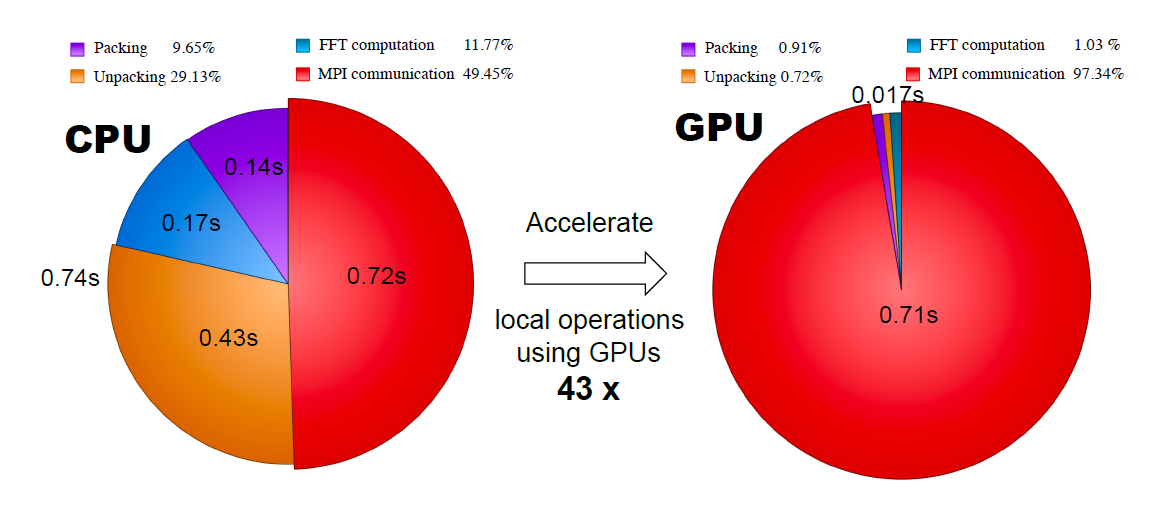
\includegraphics[width=\linewidth, keepaspectratio]{../res/speedup.png}
	\end{figure}
	\begin{itemize}
		\item $\frac{0.14s+0.17s+0.42s+0.72s}{0.017s+0.71s}=200,8\% \rightarrow$  2-fache Beschleunigung
		\item Kommunikationszeit nur vernachlässigbare Änderung
		\item rechte Seite graphisch nicht akkurat dargestellt!
	\end{itemize}
}
\frame
{
	\frametitle{Bottleneck: Kommunikation}
	Nach der Beschleunigung ist der  Zeitanteil der Kommunikation:\\
	$$\frac{0.71s}{0.71s+0.017}\approx97,6\%$$
	$\implies$ Bottleneck in der Kommunikation\\
	\large Was tun? \normalsize
}
\frame
{
	\frametitle{Was tun?}
	Konzeptionell 2 Ansätze:
	\begin{itemize}
		\item Option1: Verwendung eines besseren Algorithmus hinsichtlich serieller Anteile und Kommunikation.
		\item Option2: Verbesserung der Kommunikationsstrategie unter Einbeziehung von Eigenschaften der Systemarchitektur.
	\end{itemize}
}
\frame
{
	\frametitle{Systemarchitektur: ORNL Summit}
	\tiny Summit Supercomputer im Oak Ridge National Laboratory, Tennessee, USA\normalsize
	\begin{figure}[h!]
		\centering
		\begin{subfigure}[t]{0.3\linewidth}
			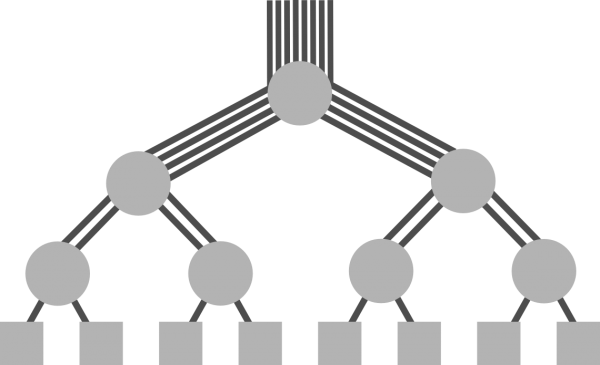
\includegraphics[width=1\linewidth]{../res/fat_tree.png}
			\footnotemark[1]
			\caption{Fat-Tree}
		\end{subfigure}
~
		\begin{subfigure}[t]{0.5\linewidth}
			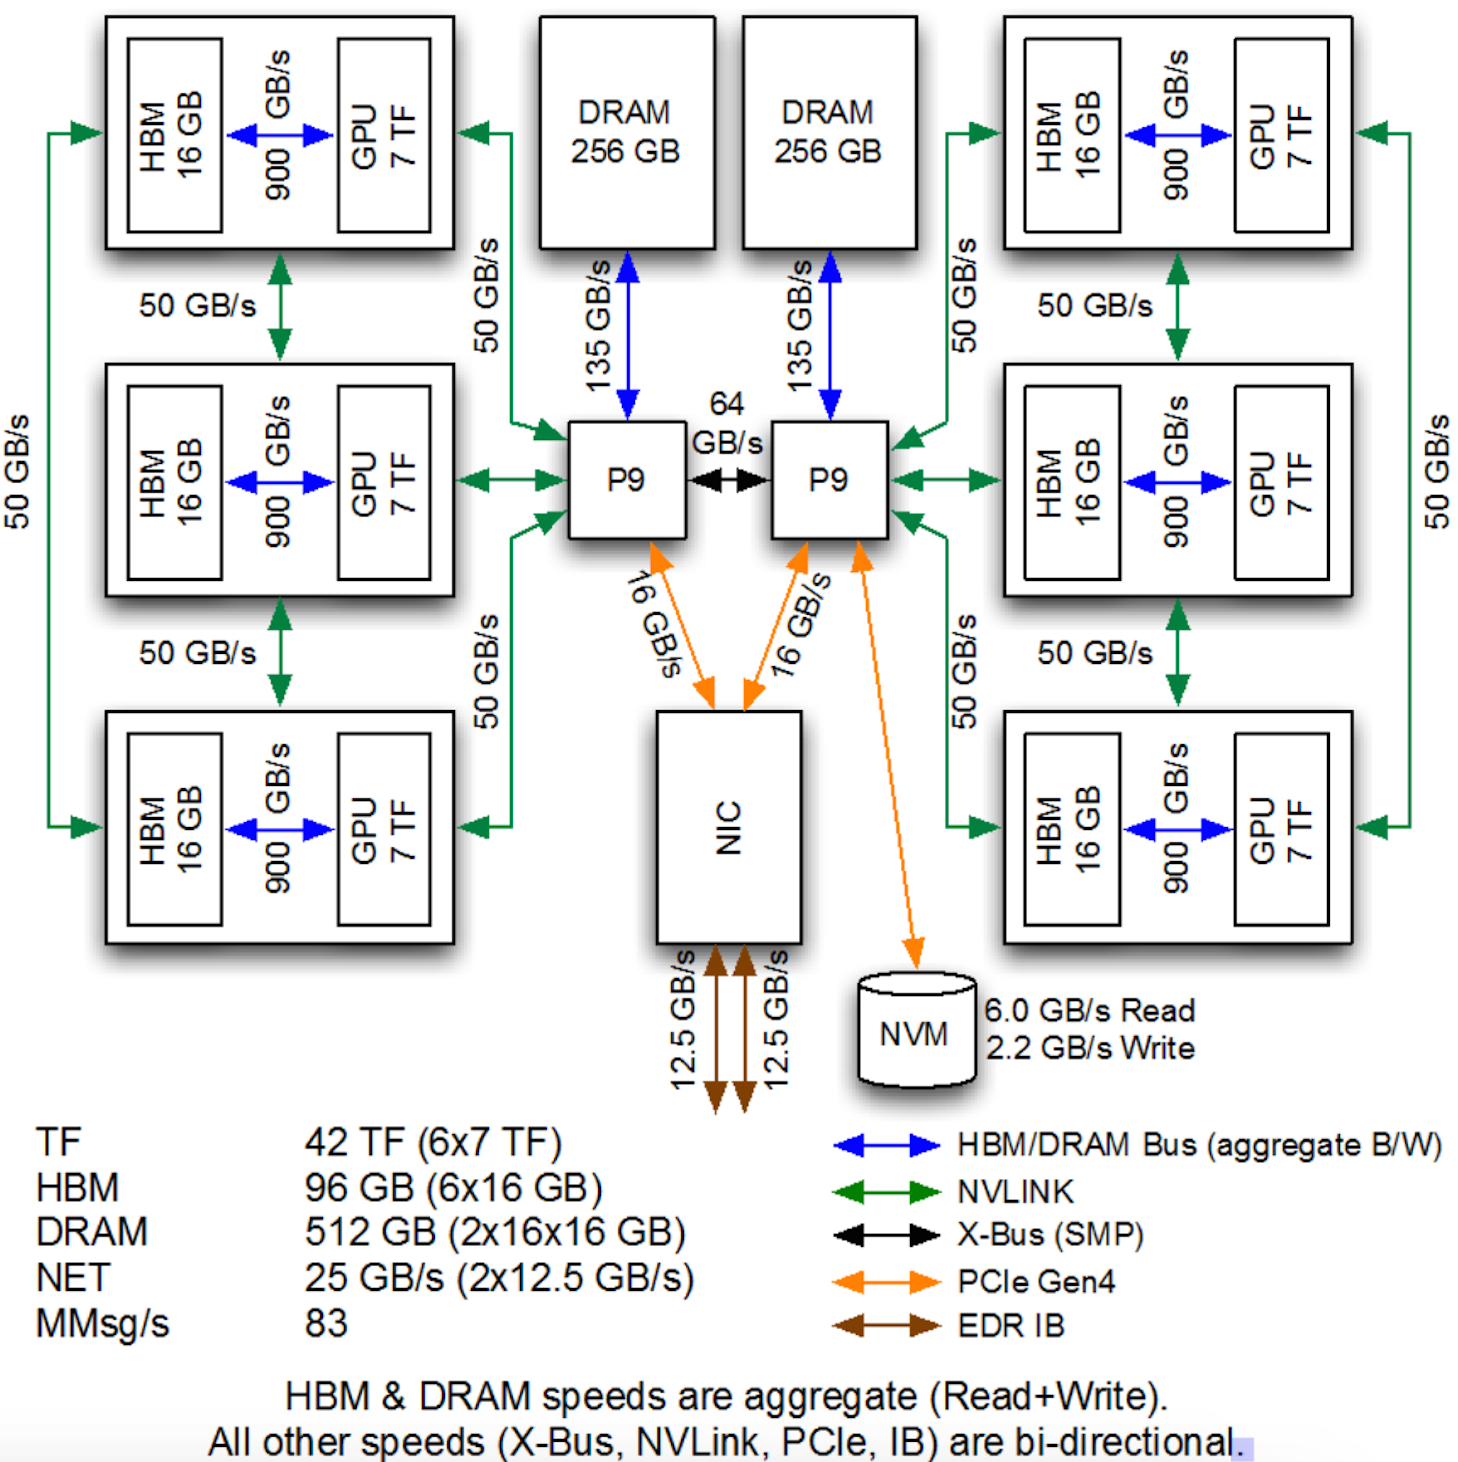
\includegraphics[width=1\linewidth]{../res/architecture.png}
			\footnotemark[2]
			\caption{Knotenarchitektur}
		\end{subfigure}
	\end{figure}

\footnotetext[1]{\tiny\url{https://clusterdesign.org/fat-trees/} am 6.2.2019\normalsize}
\footnotetext[2]{\tiny Shajek H., Tomov S., Ayala A., Haidar A., Dongarra J:\\{\sl GPUDirect MPI Communications and Optimizations to Accelerate FFTs on Exascale Systems};\\EuroMPI ’19 Posters, September 11-13, 2019, Zurich, Switzerland}
\normalsize
}

\frame
{
	\frametitle{MPI/CUDA}
\begin{itemize}
	\item[] MPI\footnotemark[1]: \textbf{M}essage \textbf{P}assing \textbf{I}nterface
	Standardisierte Kommunikationsschnittstelle zwischen Prozessen, hier im Kontext von Multiprozessorsystemen
\item[] CUDA\footnotemark[2]: Parallele Berechnungsplattform un Programmiermodel von NVIDIA für allgemeine Berechnungen auf NVIDIA GPUs.
\end{itemize}
	\footnotetext[2]{https://developer.nvidia.com/cuda-zone}
}
\frame
{
	\frametitle{NVLink}
	\begin{figure}
	\begin{subfigure}[t]{0.4\linewidth}
			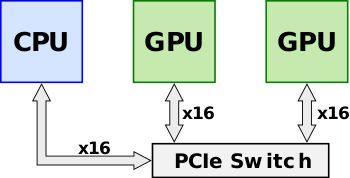
\includegraphics[width=1\linewidth]{../res/nvlink0.png}
			\caption{Traditionelle Architektur}
			\footnotemark[1]
	\end{subfigure}
~
	\begin{subfigure}[t]{0.4\linewidth}
			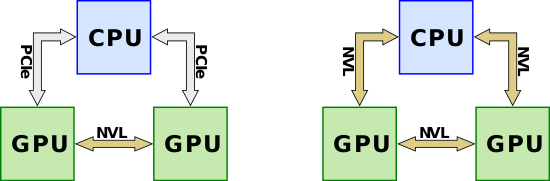
\includegraphics[width=1\linewidth]{../res/nvlink1.png}
			\caption{NVLink Architektur}
			\footnotemark[1]
		\end{subfigure}
	\end{figure}
	Stichwörter: GPUDirect (Remote Direct Memory Access), CUDA-aware MPI
	\footnotetext[1]{https://en.wikichip.org/wiki/nvidia/nvlink}
}

\frame
{
	\frametitle{Ermittlung tatsächlicher Bandbreiten}
	$\rightarrow$ Benchmarks nach Option 2
	\begin{figure}[h!]
		\centering
		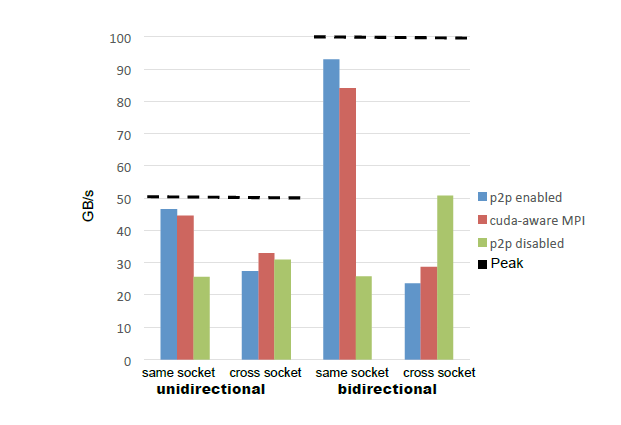
\includegraphics[width=0.7\linewidth, keepaspectratio]{../res/bench0.png}
	\footnotemark[1]
	\end{figure}
\footnotetext[1]{\tiny Shajek H., Tomov S., Ayala A., Haidar A., Dongarra J:\\{\sl GPUDirect MPI Communications and Optimizations to Accelerate FFTs on Exascale Systems};\\EuroMPI ’19 Posters, September 11-13, 2019, Zurich, Switzerland}
}
\frame
{
	\frametitle{Untersuchung verschiedener Kommunikationsstrategien}
	nach Option 2
	\begin{figure}[h!]
		\centering
		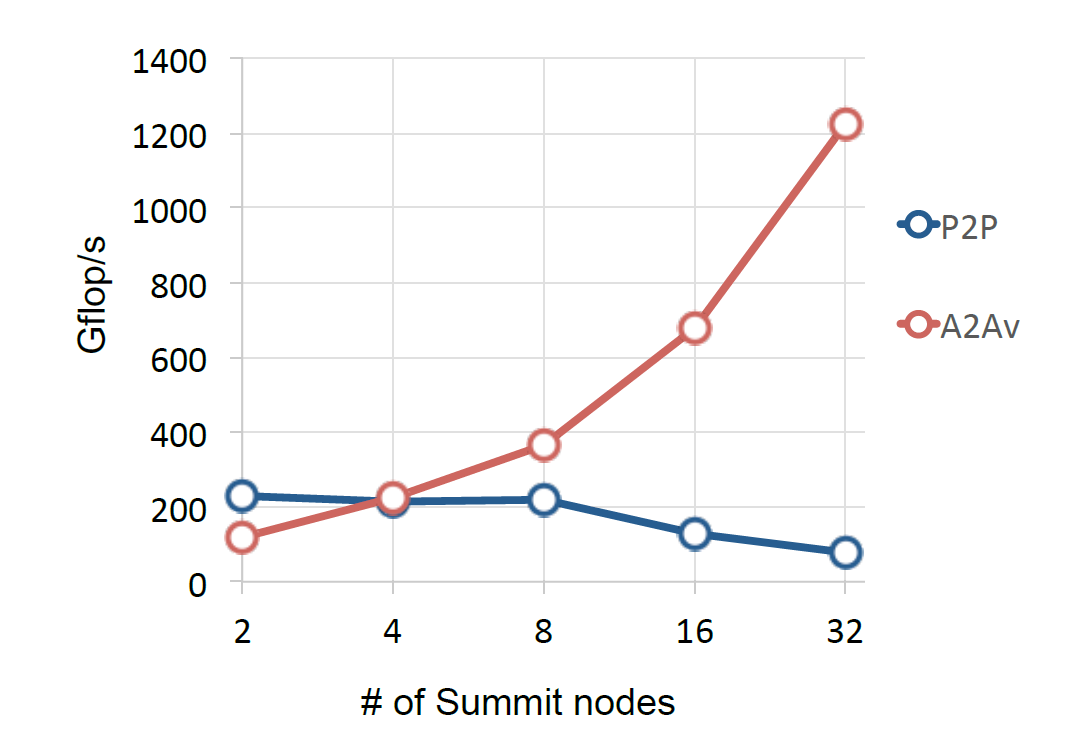
\includegraphics[width=0.7\linewidth, keepaspectratio]{../res/bench.png}
		\footnotemark[1]
	\end{figure}
\footnotetext[1]{\tiny Shajek H., Tomov S., Ayala A., Haidar A., Dongarra J:\\{\sl GPUDirect MPI Communications and Optimizations to Accelerate FFTs on Exascale Systems};\\EuroMPI ’19 Posters, September 11-13, 2019, Zurich, Switzerland}
}
\frame
{
	\frametitle{Algorithmische Änderungen: Slabs}
	nach Option 1
	\begin{figure}[h!]
		\centering
		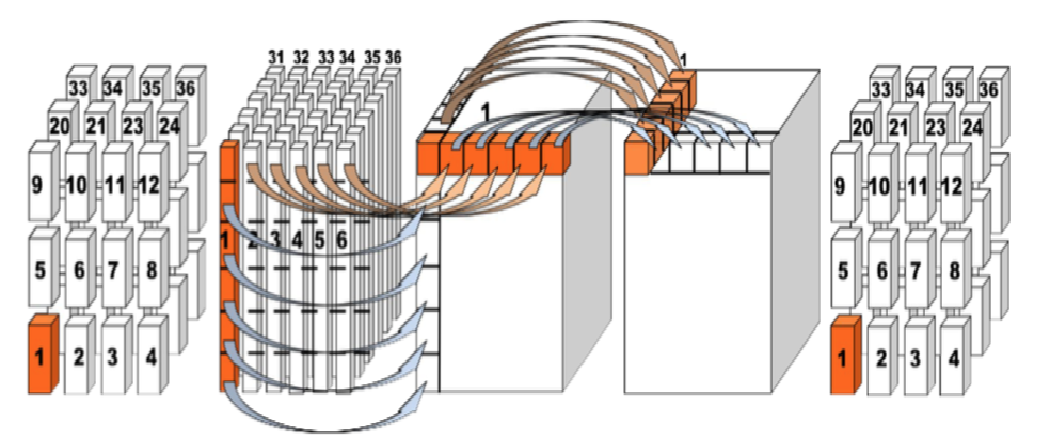
\includegraphics[width=0.7\linewidth, keepaspectratio]{../res/algo.png}
		\footnotemark[1]
	\end{figure}
	1D\textit{pencil} $\rightarrow$ 2D\textit{slabs} Übertragungsgröße
	$(TransformX,TransformY,TransformZ,MoveBack)\rightarrow(TransformY,TransformZ,MoveBack)$
	Theoretisch: $25\%$ Ersparnis

\footnotetext[1]{\tiny Shajek H., Tomov S., Ayala A., Haidar A., Dongarra J:\\{\sl GPUDirect MPI Communications and Optimizations to Accelerate FFTs on Exascale Systems};\\EuroMPI ’19 Posters, September 11-13, 2019, Zurich, Switzerland}
}

\frame
{
	\frametitle{Algorithmische Änderungen: Slabs}
	\begin{figure}[h!]
		\centering
		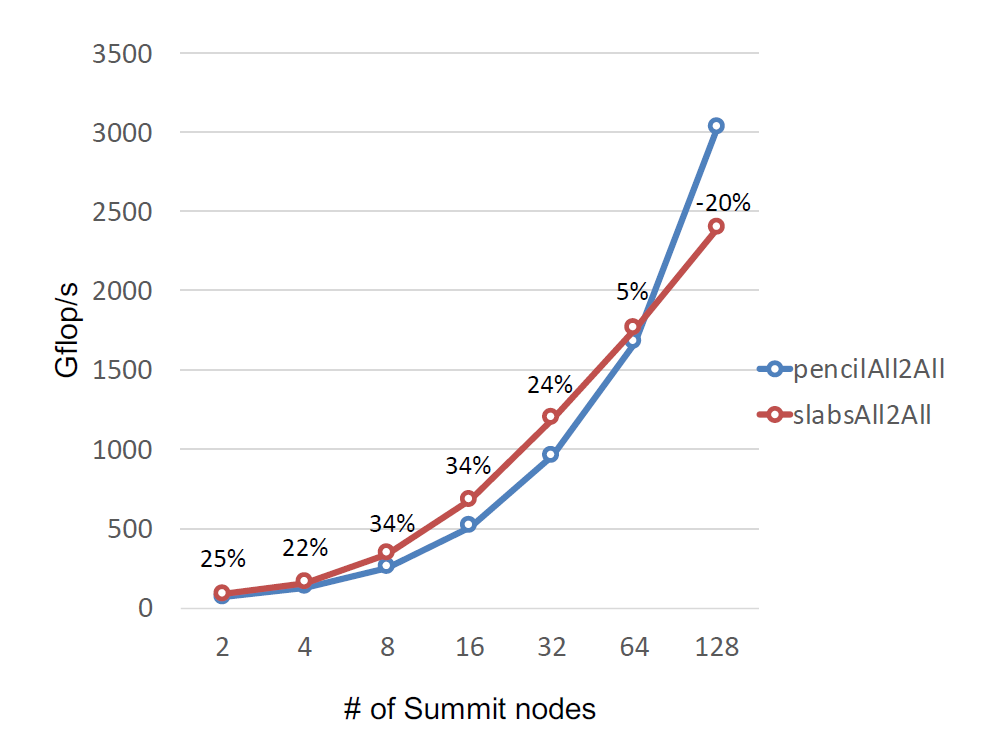
\includegraphics[width=0.7\linewidth, keepaspectratio]{../res/bench2.png}
		\footnotemark[1]
	\end{figure}
	Nachteil: Quadratischer Speicherverbrauch pro Knoten
	
\footnotetext[1]{\tiny Shajek H., Tomov S., Ayala A., Haidar A., Dongarra J:\\{\sl GPUDirect MPI Communications and Optimizations to Accelerate FFTs on Exascale Systems};\\EuroMPI ’19 Posters, September 11-13, 2019, Zurich, Switzerland}
}
\frame
{
	\frametitle{Dynamische Analysen}
	Dynamische Analysen hinsichtlich
	\begin{itemize}
		\item Speicherverbrauch
		\item Rechenlast
	\end{itemize}
	zur optimalen Auslastung und Aufteilung auf die Einheiten von Rechenressourcen vor der Ausführung des Algorithmus
	\begin{enumerate}
		\item{Knoten}
		\item{Sockel}
		\item{Prozessor}
	\end{enumerate}
	$\implies$ Vermeidung unnötiger Kommunikation oder Kommunikation über langsame Kommunikationswege.
}
